\documentclass{standalone}
\usepackage{tikz}
\usepackage{ctex,siunitx}
\setCJKmainfont{Noto Serif CJK SC}
\usepackage{tkz-euclide}
\usepackage{amsmath}
\usepackage{wasysym}
\usetikzlibrary{patterns, calc}
\usetikzlibrary {decorations.pathmorphing, decorations.pathreplacing, decorations.shapes,}
\begin{document}
\small
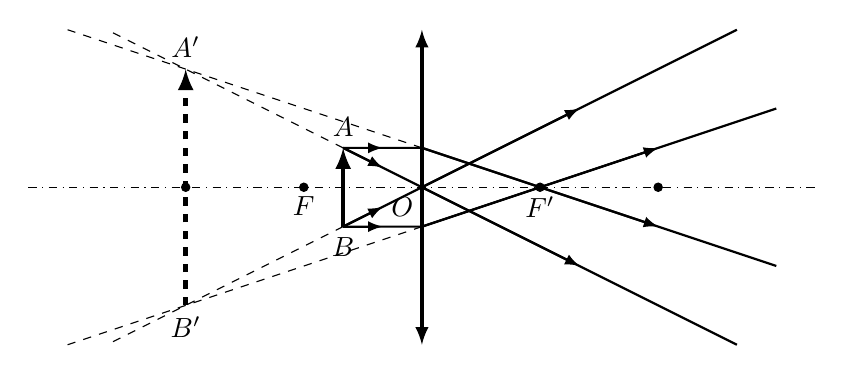
\begin{tikzpicture}[>=latex,scale=1]
  \draw[<->, very thick ] (0,2)--(0,-2);
  \draw[dashdotted](-5,0)--(5,0);
  \node at (-1.5,0)[below]{$F$};\node at (1.5,0)[below]{$F'$};\node at (-.25,-.25){$O$};
  \draw [thick](-1,.5)--(0,.5)--(1.5,0)--(4.5,-1); 
  \draw [thick](-1,-.5)--(0,-.5)--(1.5,0)--(4.5,1); 
  \draw [thick](-1,.5)--(0,0)--(4,-2);
  \draw [thick](-1,-.5)--(0,0)--(4,2);
  \draw [->, ultra thick, >=latex] (-1,-.5)node[below]{$B$}--(-1,.5)node[above]{$A$};
  \draw[dashed] (0,.5)--(-4.5, 2);   \draw[dashed] (0,-.5)--(-4.5, -2);
  \draw[dashed] (-1,.5)--(-4, 2);   \draw[dashed] (-1,-.5)--(-4, -2);
  \draw [fill=black] (-1.5,0) circle (1.5pt);
  \draw [fill=black] (1.5,0) circle (1.5pt);
  \draw [fill=black] (-3,0) circle (1.5pt);
  \draw [fill=black] (3,0) circle (1.5pt);
  \draw [->, ultra thick, >=latex, dashed] (-3,-1.5)node[below]{$B'$}--(-3,1.5)node[above]{$A'$};
  \draw [->,  thick, >=latex](-1,.5)--(-.5,.5);  \draw [->,  thick, >=latex](0,.5)--(3,-.5);
  \draw [->,  thick, >=latex](-1,-.5)--(-.5,-.5); \draw [->,  thick, >=latex](0,-.5)--(3,.5);
  \draw [->,  thick, >=latex](0,0)--(2,-1);    \draw [->,  thick, >=latex](0,0)--(2,1);
  \draw [->,  thick, >=latex](-1,.5)--(-.5,.25);\draw [->,  thick, >=latex](-1,-.5)--(-.5,-.25);
\end{tikzpicture}
\end{document}